\documentclass{article}
\usepackage{jfrExamplee}
\usepackage{graphicx}
\usepackage{apalike}
\usepackage{setspace}

%% Uncomment line below for double spacing
%\doublespacing

%this template built off template for NIPS 2004

\title{A Single Wheel Test Rig for Ocean World Rovers}

\author{
Athul Pradeepkumar Girija\thanks{ Use footnote for providing further information
about author (webpage, alternative address). Acknowledgments to
funding agencies should go in the \textbf{Acknowledgments} section
at the end of the paper.} \\
School of Aeronautics and Astronautics\\
Purdue University\\
West Lafayette, IN 47907 \\
\texttt{apradee@purdue.edu} \\
\And
Ye Lu \\
School of Aeronautics and Astronautics \\
Purdue University \\
West Lafayette, IN 47907 \\
\texttt{yelu@purdue.edu} \\
\And
Archit Arora \\
School of Aeronautics and Astronautics \\
Purdue University \\
West Lafayette, IN 47907 \\
\texttt{arora31@purdue.edu} \\
\And
Rachana Agrawal \\
School of Aeronautics and Astronautics \\
Purdue University \\
West Lafayette, IN 47907 \\
\texttt{agrawa77@purdue.edu} \\
\And
Maxim de Jong \\
Thin Red Line Aerospace \\
Chilliwack, British Columbia\\ V2R 5M3, Canada\\
\texttt{maxim@thin-red-line.com} \\
\And
Matt Kent \\
Materials Science and Engineering\\
Smithers \\
Ravenna, Ohio 44266\\
\texttt{mkent@smithers.com} \\
\And
Sarag J. Saikia \\
School of Aeronautics and Astronautics \\
Purdue University \\
West Lafayette, IN 47907 \\
\texttt{ssaikia@purdue.edu} \\
\And
James M. Longuski \\
School of Aeronautics and Astronautics \\
Purdue University \\
West Lafayette, IN 47907 \\
\texttt{longuski@purdue.edu} \\
}

% The \author macro works with any number of authors. There are two commands
% used to separate the names and addresses of multiple authors: \And and \AND.
%
% Using \And between authors leaves it to \LaTeX{} to determine where to break
% the lines. Using \AND forces a linebreak at that point. So, if \LaTeX{}
% puts 3 of 4 authors names on the first line, and the last on the second
% line, try using \AND instead of \And before the third author name.

\begin{document}

\maketitle

\begin{abstract}
"Sed ut perspiciatis unde omnis iste natus error sit voluptatem accusantium doloremque laudantium, totam rem aperiam, eaque ipsa quae ab illo inventore veritatis et quasi architecto beatae vitae dicta sunt explicabo. Nemo enim ipsam voluptatem quia voluptas sit aspernatur aut odit aut fugit, sed quia consequuntur magni dolores eos qui ratione voluptatem sequi nesciunt. Neque porro quisquam est, qui dolorem ipsum quia dolor sit amet, consectetur, adipisci velit, sed quia non numquam eius modi tempora incidunt ut labore et dolore magnam aliquam quaerat voluptatem. Ut enim ad minima veniam, quis nostrum exercitationem ullam corporis suscipit laboriosam, nisi ut aliquid ex ea commodi consequatur? Quis autem vel eum iure reprehenderit qui in ea voluptate velit esse quam nihil molestiae consequatur, vel illum qui dolorem eum fugiat quo voluptas nulla pariatur?"
\end{abstract}

\section{Introduction}

This document provides a sample template that can be used for
submission of articles to the Journal of Field Robotics.

The style files for JFR, are available on the World Wide Web at
\begin{center}
   http://journalfieldrobotics.org/templates/
\end{center}
The file jfrExample.ps (or jfrExample.pdf) contains these
instructions and illustrates the various formatting requirements
your JFR paper must satisfy. \LaTeX{} users can choose between two
style files: jfrExample.sty (to be used with \LaTeX{} version 2.09)
and jfrExamplee.sty (to be used with \LaTeX{}2e). The file
jfrExample.tex may be used as a ``shell'' for writing your paper.
All you have to do is replace the author, title, abstract, and text
of the paper with your own.

The formatting instructions contained in these style files are summarized in
sections \ref{gen_inst}, \ref{headings}, and \ref{others} below.

\section{General formatting instructions}
\label{gen_inst}

The main text of your paper should be in a single column textbox 6.5
inches by 9 inches. Regular text should be in a 12 point font.
Paragraphs should not be indented, and should be separated by a
single line space.

Please pay attention to the instructions in section \ref{others}
regarding figures, tables, acknowledgments, and references.

\section{Headings: first level}
\label{headings}

First level headings are lower case (except for first word and
proper nouns), flush left, bold and in point size 14. One line space
before the first level heading and 1/2~line space after the first
level heading.

\subsection{Headings: second level}

Second level headings are lower case (except for first word and
proper nouns), flush left, bold and in point size 12. One line space
before the second level heading and 1/2~line space after the second
level heading.

\subsubsection{Headings: third level}

Third level headings are lower case (except for first word and
proper nouns), flush left, bold and in point size 12. One line space
before the third level heading and 1/2~line space after the third
level heading.

\section{Citations, figures, tables, references}
\label{others}

If not using the  latex template, please try to produce citations,
references, and figure captions as close as possible to the example.

\subsection{Citations within the text}

Citations should follow the APA style \cite{apa}. Unlike many
scientific papers, this requires in text citation of authors' names
and date of work. The corresponding references are to be listed in
alphabetical order using APA reference style at the end of the
paper, in the \textbf{References} section. Example references are
given in this template for books with one author \cite{baxter},
conference papers \cite{binh}, journal articles \cite{baldwin}, and
books with editors \cite{stock}. For electronic references without
authors, the reference is cited using the web page title. The
University of Wisconsin Writing Center provides a good resource for
questions about the APA style \cite{wisconsin}.

\subsection{Footnotes}

Indicate footnotes with a number\footnote{Sample of the first
footnote} in the text. Place the footnotes at the bottom of the page
on which they appear. Precede the footnote with a horizontal rule of
2~inches.\footnote{Sample of the second footnote}

\subsection{Figures}

All artwork must be neat, clean, and legible. Lines should be dark
enough for purposes of reproduction; art work should not be
hand-drawn. We recommend using either the jpg or the embedded
postscript format for images and the tiff format for line drawings.
If the figures contain graphs, please ensure that the axis labels
are legible when printed. Figure number and caption always appear
after the figure. Place one line space before the figure caption,
and one line space after the figure. The figure caption is lower
case (except for first word and proper nouns); figures are numbered
consecutively.

Make sure the figure caption does not get separated from the figure.
Leave sufficient space to avoid splitting the figure and figure caption.

\begin{figure} [h]
    \centering
    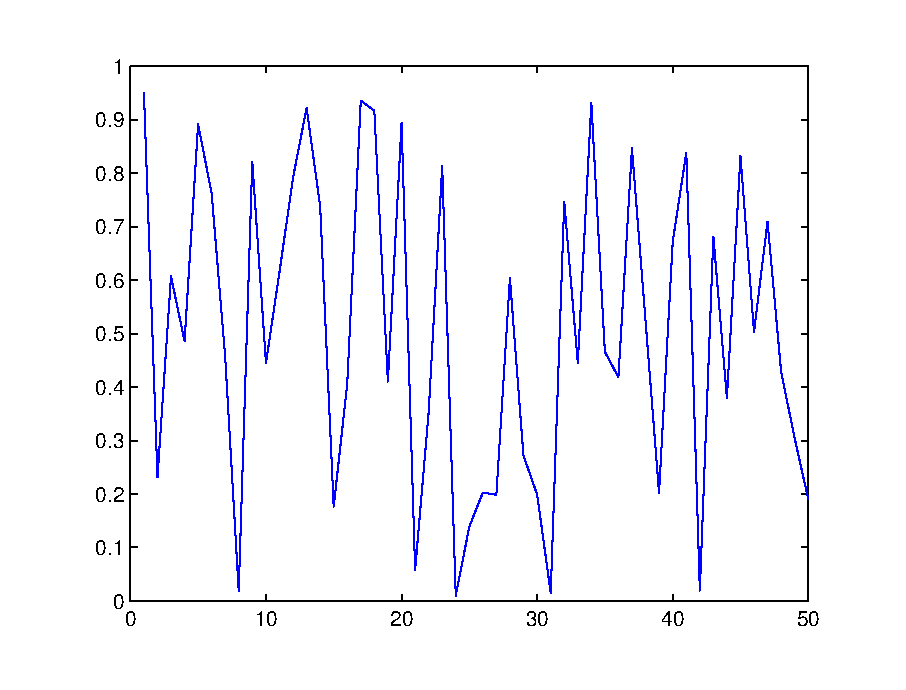
\includegraphics[height=2.0in]{g1}
    \hspace{.2in}
    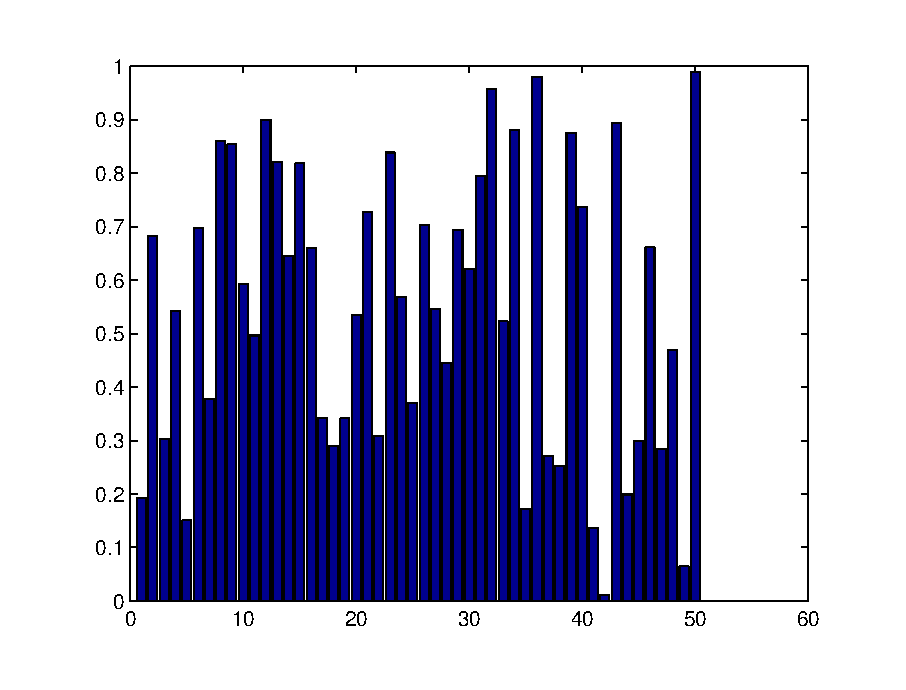
\includegraphics[height=2.0in]{g2}
    \caption{Line graph of random numbers (left) and bar graph of random numbers (right)}
    \label{fig:sampleFigure}
\end{figure}

\subsection{Tables}

All tables must be centered, neat, clean and legible. Do not use hand-drawn
tables. Table number and title always appear before the table. See
Table~\ref{sample-table}.

Place one line space before the table title, one line space after the table
title, and one line space after the table. The table title must be lower case
(except for first word and proper nouns); tables are numbered consecutively.

\begin{table}[t]
\caption{Sample table title} \label{sample-table}
\begin{center}
\begin{tabular}{|c|c|c|c|c|c|}
  \hline
% after \\: \hline or \cline{col1-col2} \cline{col3-col4} ...
   & $k_{g}$ & $k_{o}$ & $c_{3}$ & $c_{4}$ & $c_{5}$ \\
  \hline\hline
  Careful/Sparse & 0.334 & 0.597 & 1.101 & 9.621 & 8.170 \\ \hline
  Careful/Dense & 3.124 & 3.195 & 1.094 & 5.899 & 7.318 \\ \hline
  Aggressive/Sparse & 0.840 & 9.153 & 2.853 & 8.274 & 0.187 \\ \hline
  Aggressive/Dense & 4.838 & 2.841 & 0.670 & 7.952 & 0.386 \\ \hline
  Hand-Tuned & 0.767 & 0.060 & 0.340 & 2.000 & 0.250 \\
  \hline
\end{tabular}
\end{center}
\end{table}

\subsection{APA Reference Style}

References follow the acknowledgments. Use an unnumbered third level
heading for the references. References must be listed in the APA
format (available at http://www.apastyle.org/). References should be
in the same font size as the paper text.

\subsubsection*{Acknowledgments}
Use unnumbered third level headings for the acknowledgments. All
acknowledgments go at the end of the paper.

\bibliographystyle{apalike}
\bibliography{jfrExampleRefs}

\end{document}